% sage_latex_guidelines.tex V1.10, 24 June 2016

\documentclass[Afour,sageh,times]{sagej}

\usepackage{moreverb,url}

\usepackage[colorlinks,bookmarksopen,bookmarksnumbered,citecolor=red,urlcolor=red]{hyperref}

\newcommand\BibTeX{{\rmfamily B\kern-.05em \textsc{i\kern-.025em b}\kern-.08em
T\kern-.1667em\lower.7ex\hbox{E}\kern-.125emX}}

% customizations
\usepackage{tabulary}
\usepackage{tabu}
\usepackage{booktabs}
\usepackage{array}
\newcommand{\ra}[1]{\renewcommand{\arraystretch}{#1}}

\def\volumeyear{2017}

\begin{document}

\runninghead{Harmon et~al.}

\title{Tangible Landscape}

\author{Brendan A Harmon\affilnum{1,2}, Anna Petrasova\affilnum{1}, Vaclav Petras\affilnum{1}, Helena Mitasova\affilnum{1}, and Ross Meentemeyer\affilnum{1}}

\affiliation{\affilnum{1}Center for Geospatial Analytics, North Carolina State University, USA\\
\affilnum{2}College of Design, North Carolina State University, USA}

\corrauth{Brendan A Harmon, 
Center for Geospatial Analytics,
North Carolina State University,
Raleigh, NC 27615, USA.}

\email{brendan.harmon@gmail.com}

\begin{abstract}
Tangible interfaces for spatial modeling
combine embodied, kinaesthetic interaction with spatial computations. 
Theoretically this should enable users to 
intuitively interact 
with multidimensional digital models of space,
offloading challenging cognitive tasks onto the body and 
computationally enhancing how they think about space.
We have designed Tangible Landscape 
-- a tangible interface powered by a geographic information system (GIS) 
that gives 3D spatial data an interactive, physical form so that 
users can naturally sense and shape it.
Tangible Landscape couples a physical and a digital model of a landscape
through real-time cycles of 
physical manipulation, 3D scanning, spatial computation, and projected feedback.
Through a series of 
3D modeling experiments 
assessed using both
quantitative and qualitative methods 
we determined that Tangible Landscape 
can improve 3D spatial performance. 
Participants produced more accurate models 
that better represented morphological features 
with tangible modeling than they did with either digital or analog, hand modeling.
\end{abstract}

\keywords{Human-computer interaction, tangible interfaces, interaction design, physical computation, embodied cognition, spatial thinking, geospatial modeling}

\maketitle


\clearpage

% ---------------------------- TEMPLATE ---------------------------- 

\begin{figure*}
%\setlength{\fboxsep}{0pt}%
%\setlength{\fboxrule}{0pt}%
\begin{center}
\end{center}
\caption{...}
\label{F1}
\end{figure*}

% ---------------------------- WATER FLOW ---------------------------- 

\begin{table*}[h]
\small\sf\centering
%
\caption{Water flow experiment: maps of per-cell statistics draped over a 3D rendering of the topography  for all participants.}
\ra{1.3}
\begin{tabular}{m{0.24\textwidth} m{0.24\textwidth} m{0.24\textwidth} m{0.24\textwidth}}
\toprule
\multicolumn{1}{c}{Reference elevation} & \multicolumn{1}{c}{Mean elevation} & \multicolumn{1}{c}{Stdev.~ of elevations} & \multicolumn{1}{c}{Stdev.~ of differences}\\
\midrule
\includegraphics[width=0.24\textwidth]{images/render_3d/participants/dem_5.png} &
\includegraphics[width=0.24\textwidth]{images/render_3d/participants/mean_dem_5.png} &
\includegraphics[width=0.24\textwidth]{images/render_3d/participants/stdev_dem_5.png} &
\includegraphics[width=0.24\textwidth]{images/render_3d/participants/stdev_regression_difference_series_5.png}\\
%
\multicolumn{1}{c}{\includegraphics[width=0.22\textwidth]{images/legends/elevation_legend_5.pdf}} &
\multicolumn{1}{c}{\includegraphics[width=0.22\textwidth]{images/legends/elevation_legend_5.pdf}} &
\multicolumn{1}{c}{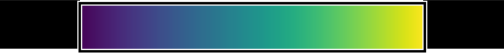
\includegraphics[width=0.22\textwidth]{images/legends/stdev_legend.pdf}} &
\multicolumn{1}{c}{\includegraphics[width=0.22\textwidth]{images/legends/stdev_diff_legend.pdf}}\\
%
\bottomrule
\end{tabular}
\label{table:water_flow_stats} 
%
\vspace*{1.5em}
%
\caption{Water flow experiment: maps of geospatial analyses draped over a 3D rendering of the topography  for all participants}
\ra{1.3}
\begin{tabular}{m{0.1\textwidth} m{0.3\textwidth} m{0.3\textwidth} m{0.3\textwidth}}
\toprule
& \multicolumn{1}{c}{Elevation} & \multicolumn{1}{c}{Water depth} & \multicolumn{1}{c}{Depth difference}\\
\midrule
%
Reference & 
\includegraphics[width=0.3\textwidth]{images/render_3d/participants/dem_5.png} &
\includegraphics[width=0.3\textwidth]{images/render_3d/participants/depth_5.png} &
\includegraphics[width=0.3\textwidth]{images/render_3d/participants/dem_difference_5.png}\\
%
Mean & 
\includegraphics[width=0.3\textwidth]{images/render_3d/participants/mean_dem_5.png} &
\includegraphics[width=0.3\textwidth]{images/render_3d/participants/mean_depth_5.png} &
\includegraphics[width=0.3\textwidth]{images/render_3d/participants/mean_depth_difference_5.png}\\
%
& 
\multicolumn{1}{c}{\includegraphics[width=0.22\textwidth]{images/legends/elevation_legend_5.pdf}} &
\multicolumn{1}{c}{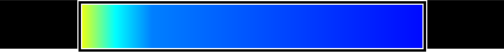
\includegraphics[width=0.22\textwidth]{images/legends/depth_legend.pdf}} &
\multicolumn{1}{c}{\includegraphics[width=0.22\textwidth]{images/legends/depth_diff_legend.pdf}}\\
%
\bottomrule
\end{tabular}
\label{table:water_flow_experiment} 
%
\vspace*{1.5em}
%
\caption{Water flow experiment: percent cells}
\ra{1.3}
\begin{tabular}{rrcccccccc}\toprule
method && \multicolumn{2}{c}{concentrated flow} & \phantom{abc}& \multicolumn{2}{c}{ridges} &
\phantom{abc} & \multicolumn{2}{c}{valleys}\\
\cmidrule{3-4} \cmidrule{6-7} \cmidrule{9-10}
&& reference & mean && reference & mean && reference & mean\\ \midrule
water flow && 3.28 & 2.26 && 1.18 & 2.99 && 4.77 & 3.70\\
\bottomrule
\end{tabular}
\label{table:water_flow_percent_cells} 
\end{table*}

\begin{table*}
\caption{Water flow experiment: comparison of 3D modeling novices and experts}
\ra{1.3}
\begin{tabular}{m{0.12\textwidth} m{0.24\textwidth} m{0.24\textwidth} m{0.24\textwidth} m{0.24\textwidth}}
\toprule
& \multicolumn{1}{c}{Elevation} & \multicolumn{1}{c}{Stdev.~ of differences} & \multicolumn{1}{c}{Water depth} & \multicolumn{1}{c}{Depth difference}\\
\midrule
%
Reference & 
\includegraphics[width=0.2\textwidth]{images/render_3d/3d_experts/dem_5.png} &
\includegraphics[width=0.2\textwidth]{images/render_3d/3d_experts/dem_difference_5.png}
&
\includegraphics[width=0.2\textwidth]{images/render_3d/3d_experts/depth_5.png} &
\includegraphics[width=0.2\textwidth]{images/render_3d/3d_experts/dem_difference_5.png}\\
%
3D novices & 
\includegraphics[width=0.2\textwidth]{images/render_3d/3d_novices/mean_dem_5.png} &
\includegraphics[width=0.2\textwidth]{images/render_3d/3d_novices/stdev_regression_difference_series_5.png} &
\includegraphics[width=0.2\textwidth]{images/render_3d/3d_novices/mean_depth_5.png} &
\includegraphics[width=0.2\textwidth]{images/render_3d/3d_novices/mean_depth_difference_5.png}\\
%
3D experts & 
\includegraphics[width=0.2\textwidth]{images/render_3d/3d_experts/mean_dem_5.png} &
\includegraphics[width=0.2\textwidth]{images/render_3d/3d_experts/stdev_regression_difference_series_5.png} &
\includegraphics[width=0.2\textwidth]{images/render_3d/3d_experts/mean_depth_5.png} &
\includegraphics[width=0.2\textwidth]{images/render_3d/3d_experts/mean_depth_difference_5.png}\\
%
& 
\multicolumn{1}{c}{\includegraphics[width=0.22\textwidth]{images/legends/elevation_legend_5.pdf}} &
\multicolumn{1}{c}{\includegraphics[width=0.22\textwidth]{images/legends/stdev_diff_legend.pdf}} &
\multicolumn{1}{c}{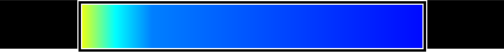
\includegraphics[width=0.22\textwidth]{images/legends/depth_legend.pdf}} &
\multicolumn{1}{c}{\includegraphics[width=0.22\textwidth]{images/legends/depth_diff_legend.pdf}}\\
%
\bottomrule
\end{tabular}
\label{table:water_flow_comparison} 
\end{table*}

\end{document}
